\section{Analysis}

\subsection{Description of the simulation}
\begin{table}[htbp]
\centering
\begin{tabular}{ c | c | c | c | c }
name of the simulation & \# of patches & total mass [M\(_\odot\)]& \makecell{mass of the \\ \ac{IMBH} [M\(_\odot\)]}& r\(_\mathrm{m}\) [pc]\\
\hline			
  SIM 1 - IMBH & 1026735 & 308533.2 & 10102 & 4.13 \\
  SIM 2 - IMBH & 1079376& 326253.4 & 8902.3 & 3.58\\
  SIM 3 - NOIMBH & 468627& 172671.3& 0 & 7.89\\
  SIM 4 - NOIMBH & 1851556& 669844.3& 0 & 5.41\\

\end{tabular}
\caption{Overview of the data of the simulations.\color{red} Question @ Paolo: Should \# of patches include IMBH? \color{black}}
\end{table}

\color{red}where simulation comes from and what it is \& description of output \color{black}\\
\\
To get a familiar with the simulation we first have a look at the scatter plot of the star positions.
\begin{figure}[htbp] 
\centering
\begin{subfigure}{0.9\textwidth}
	\centering
  	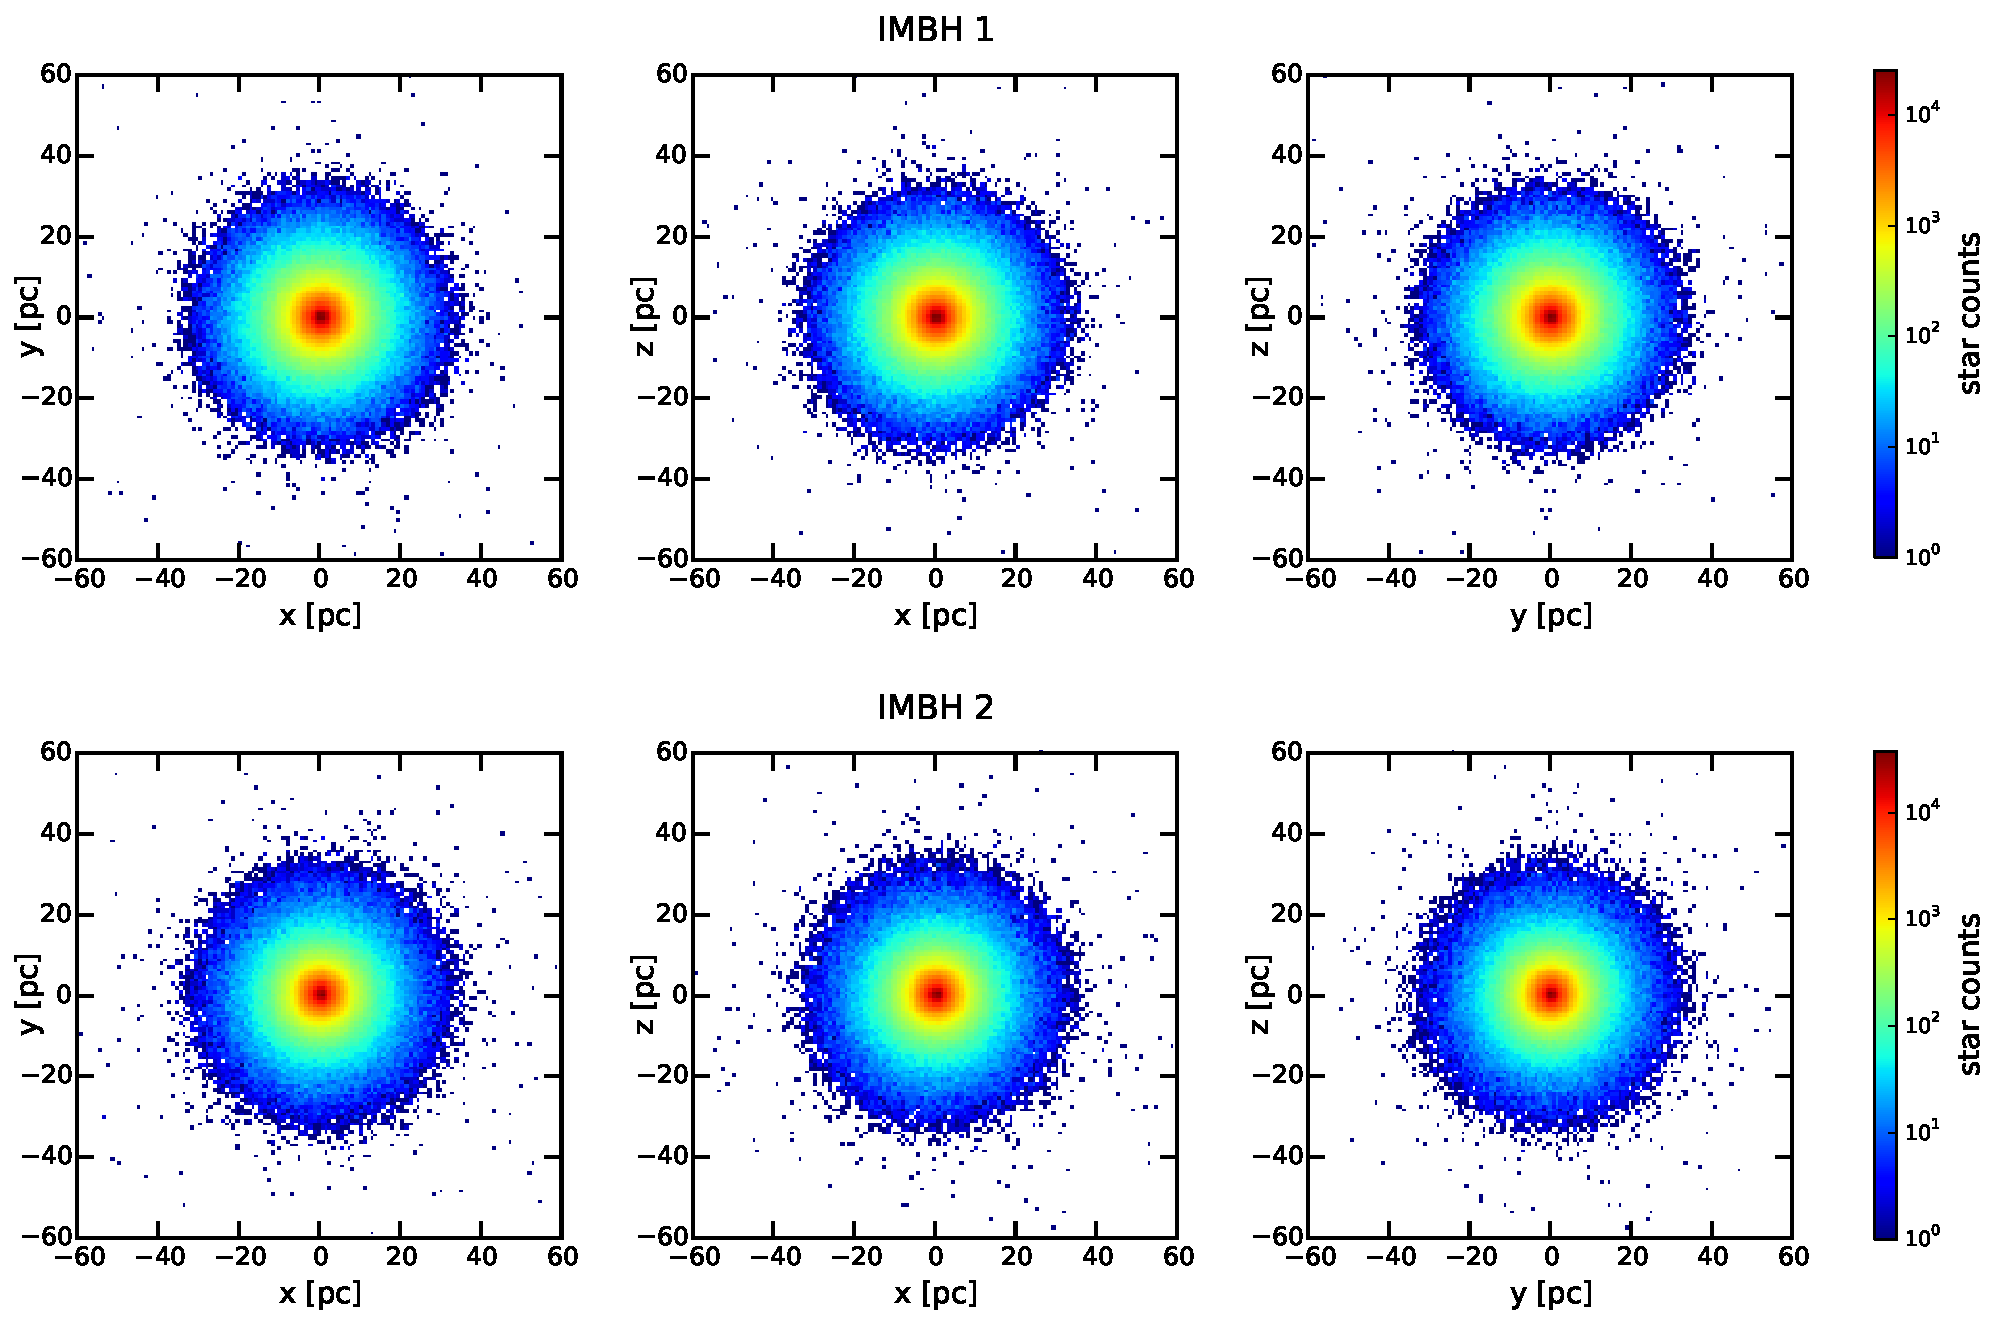
\includegraphics[width=\textwidth]{Plots/position_scatter_plot_IMBH.pdf}
  	\caption{SIM 1. The \ac{GC} is spread until 100 pc with most of the stars located in the inner 40 pc.}
 	\label{fig:pos_scat_IMBH}
\end{subfigure}
\\
\begin{subfigure}{0.9\textwidth}
	\centering
  	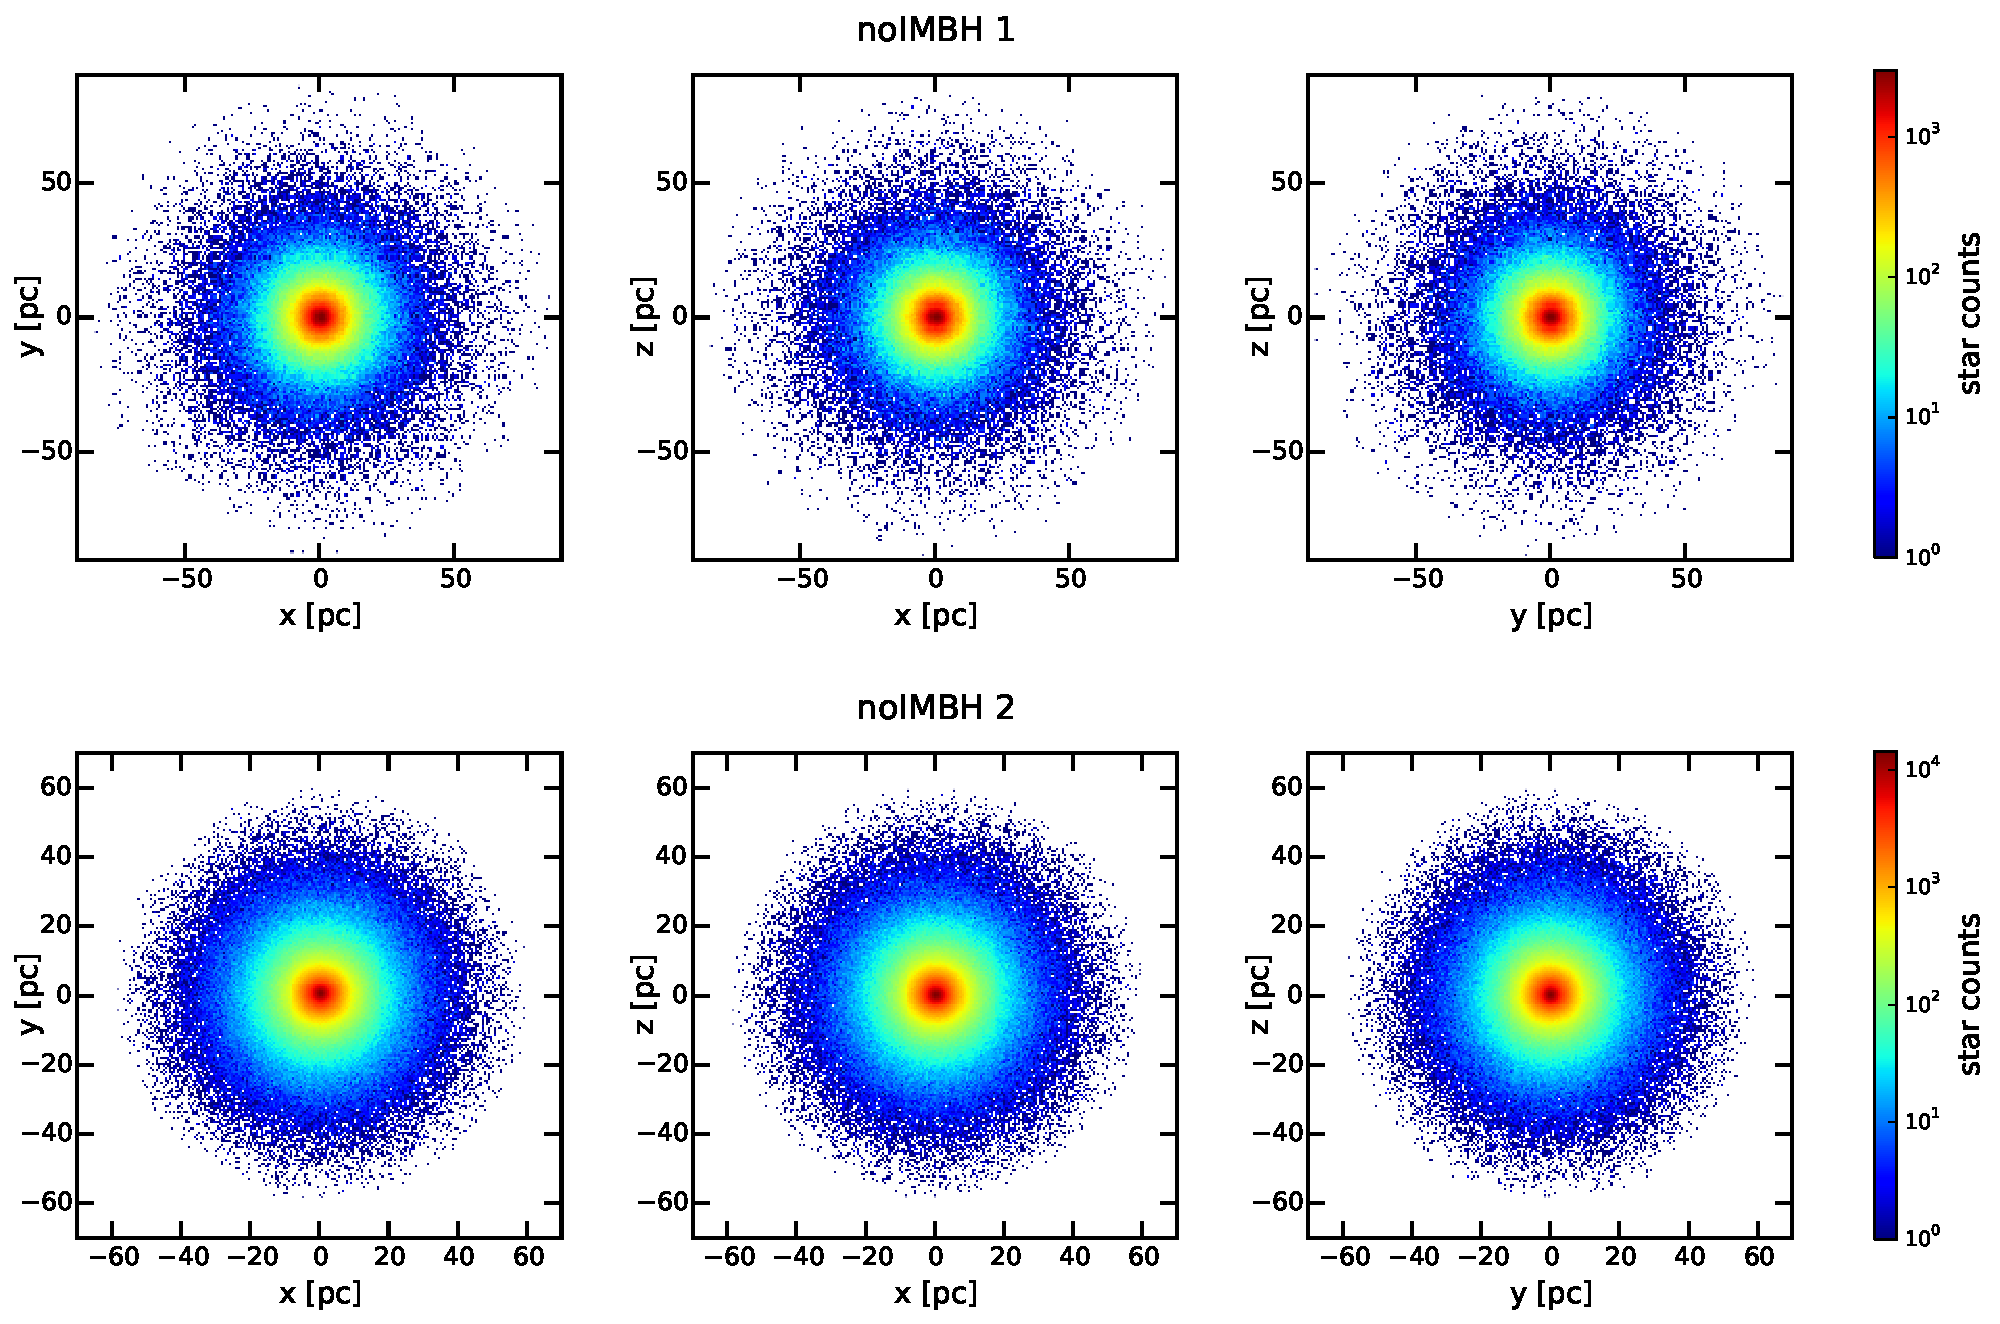
\includegraphics[width=\textwidth]{Plots/position_scatter_plot_noIMBH.pdf}
  	\caption{SIM 3. The \ac{GC} is spread until 90 pc.}
 	\label{fig:pos_scat_noIMBH}
\end{subfigure}

\caption{Position scatter plots. The stars are distributed spherically with most of the stars in the inner part. The stars of the \ac{GC} with \ac{IMBH} are less spread in the outer parts despite very few which are far outside. In the \acp{GC} without \ac{IMBH} the stars in the outer part are less accumulated but the furthermost stars still in the main sphere.}
\label{fig:position_scatter}
\end{figure}

\begin{figure}[htbp] 
\centering
\begin{subfigure}{0.95\textwidth}
	\centering
  	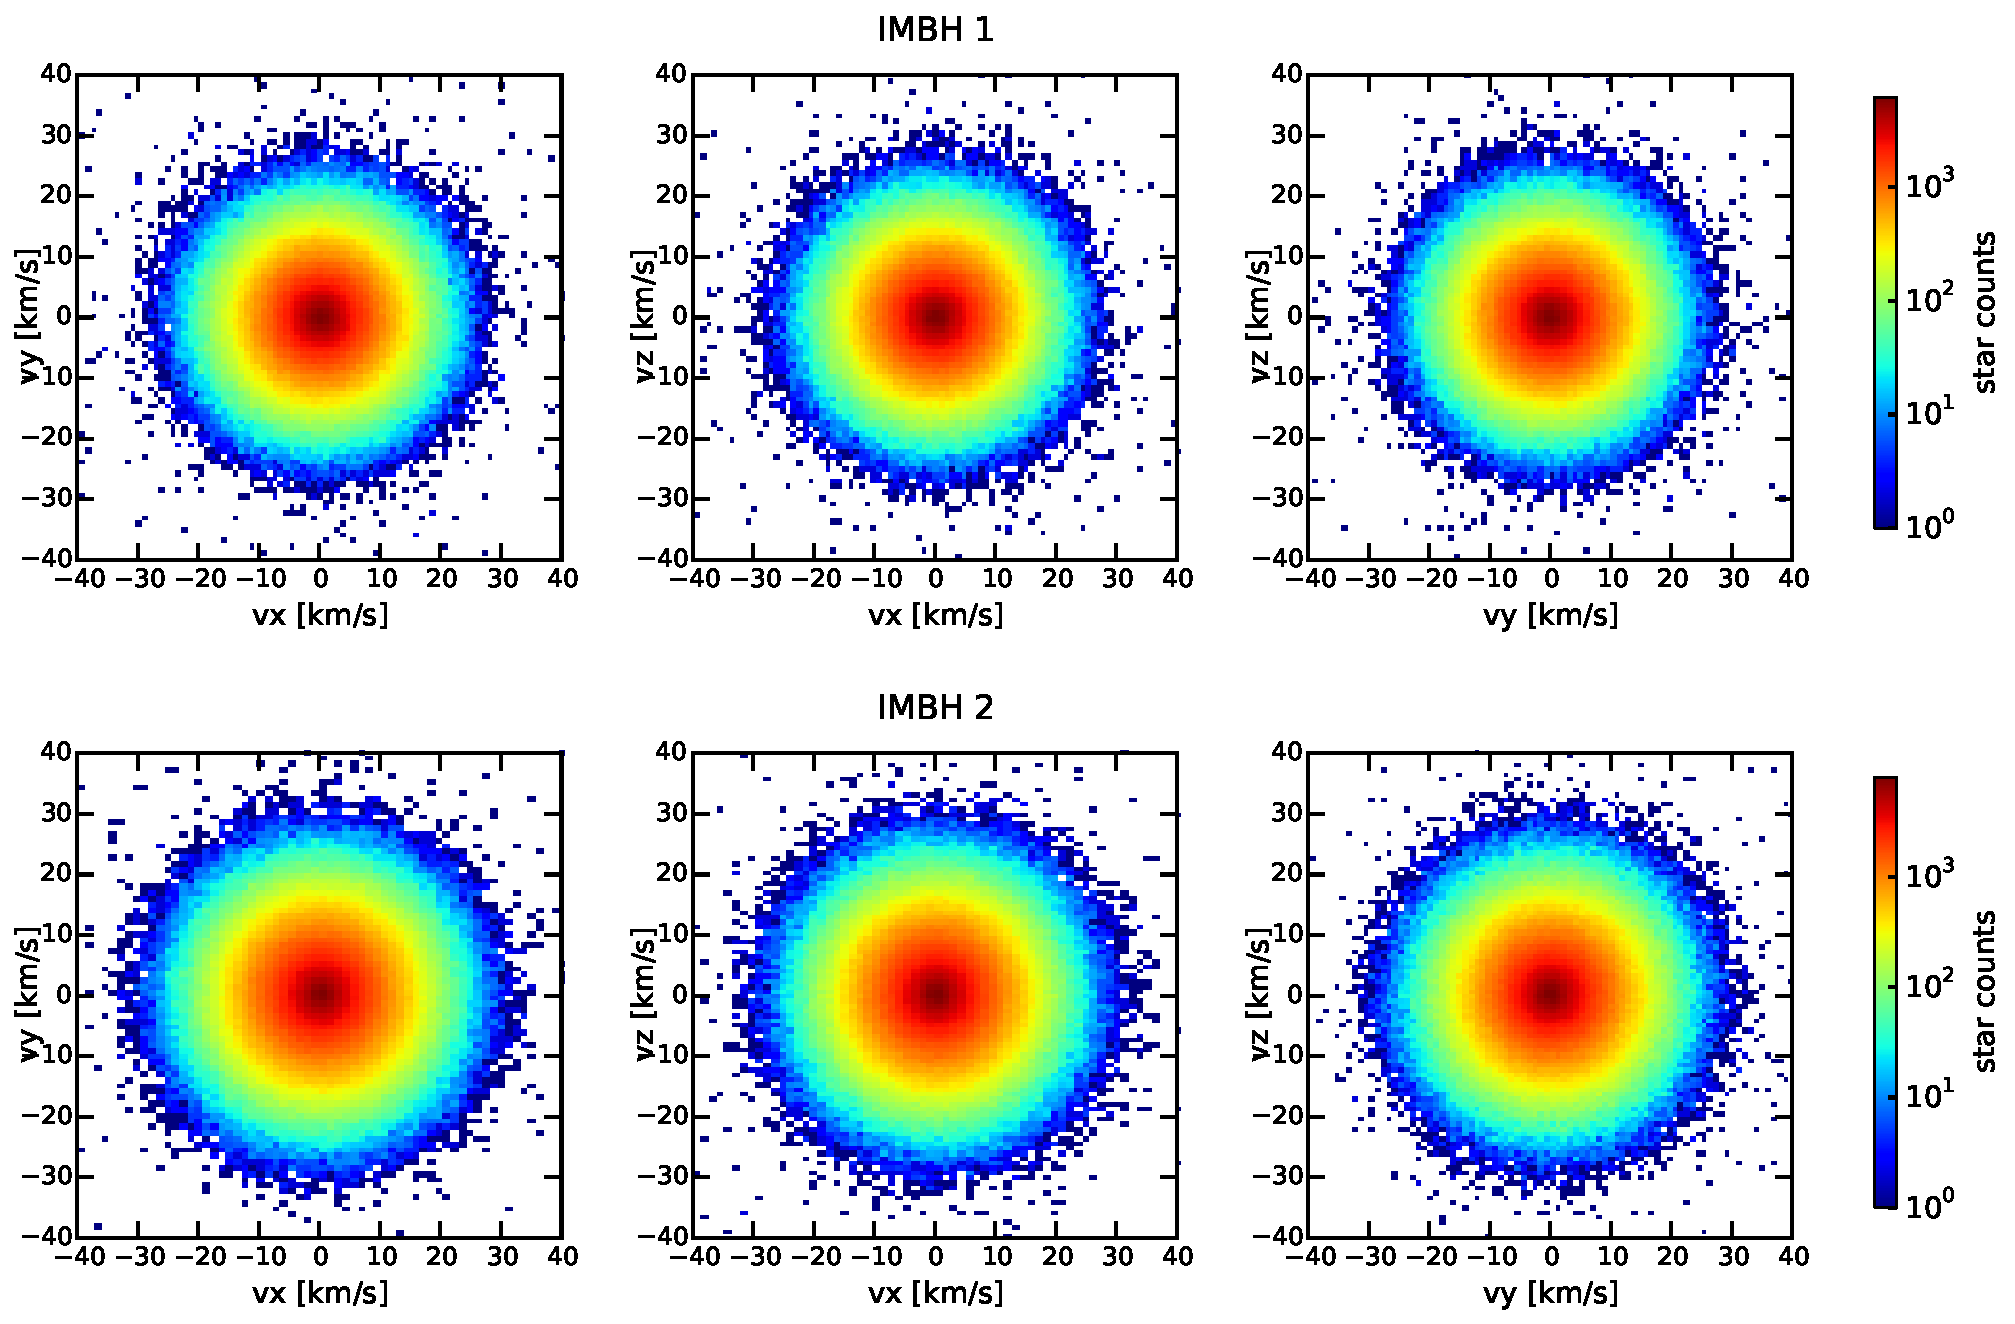
\includegraphics[width=\textwidth]{Plots/velocity_scatter_IMBH.pdf}
  	\caption{SIM 1. The stars' velocities are spread until 120 km/s with most of them reaching 30 km/s.}
 	\label{fig:vel_scat_IMBH}
\end{subfigure}
\\
\begin{subfigure}{0.95\textwidth}
	\centering
  	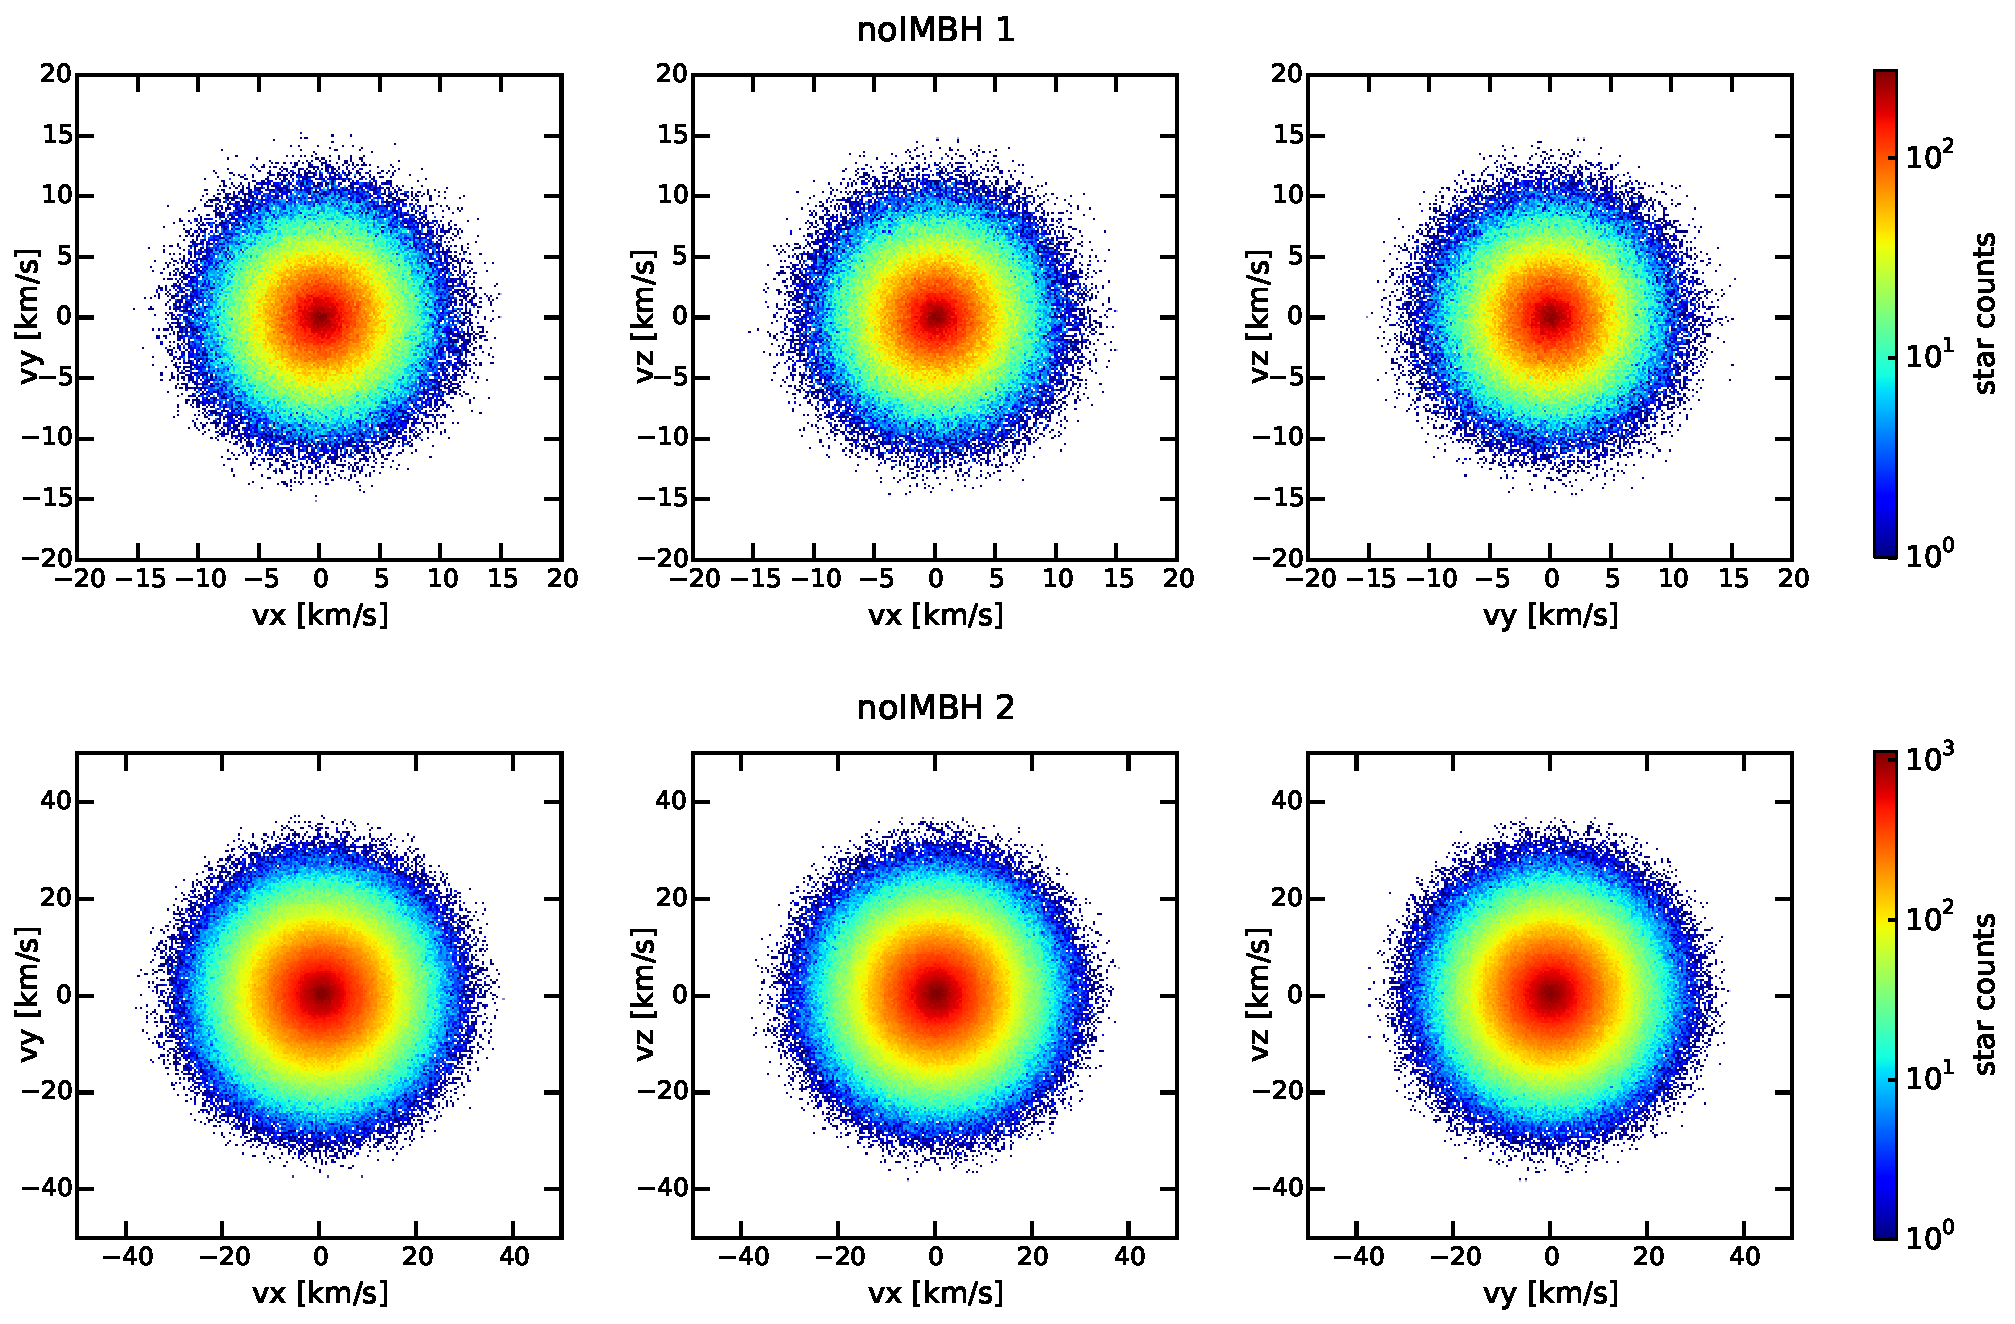
\includegraphics[width=\textwidth]{Plots/velocity_scatter_noIMBH.pdf}
  	\caption{SIM 3. The stars' velocities are spread until 15 km/s.}
 	\label{fig:vel_scat_noIMBH}
\end{subfigure}

\caption{Velocity scatter plots. The velocities are spherically distributed. Most of the stars have low or no velocity while a few have high velocities in different directions. Like the star distribution the velocity distribution of the \ac{GC} with \ac{IMBH} has some velocities outside the main sphere whereas the \acp{GC} without \ac{IMBH} contains all velocities inside the main shell.}
\label{fig:velocity_scatter}
\end{figure}
\color{red} include same plot with velocities!! \color{black}\\
As we said in section \ref{sec2.1} it is important to test the sphericity of a system. We will do this by splitting the \ac{GC} into octants and compare their mass \color{red} or number since we will introduce mass density plots only later \color{black} density \color{red} mass density sphericity plots\color{black}. As you see they're acceptable overlaying \color{red} within their errors. \color{black}
\\
As mentioned in \ref{sec1.2} the \ac{CMD} is showing a star's evolution stage dependend on its position. If you do not know age or metallicity of the system you can fit isochrones on the \ac{CMD}. Isochrones are curves of evolutionary stages of stars having the same age and metallicity but different masses. We plot several to our \ac{CMD} to determine which one fits best. This will give us the age and the metallicity of the system. \color{red} cmd with isocrones plots \color{black}


\subsection{Investigation in phase space}

First we will investigate the \ac{GC} in phase space for the set of simulations that w will use throughout this work. We will start with the velocity dispersion and the anisotropy parameter then we will have a density profile and from that get the potential. \color{red} for all 4 simulations or only for the first with IMBH? or with on plot containing two or all of them? \color{black}

\subsubsection{Velocity dispersion}
With (1) from section \ref{sec2.1} we can calculate the velocity dispersion for each coordinate \(r,\theta,\phi\). For every bin we take the same amount of stars and calculate the dispersion. To compare both simulations we plot the dispersion over the effective radius. The half mass radius of the simulation with \ac{IMBH} is 4.1pc and of the simulation without \ac{IMBH} it is 7.9pc. 
\begin{figure*}[htbp]
	\centering
	\begin{subfigure}{0.475\textwidth}
		\centering
		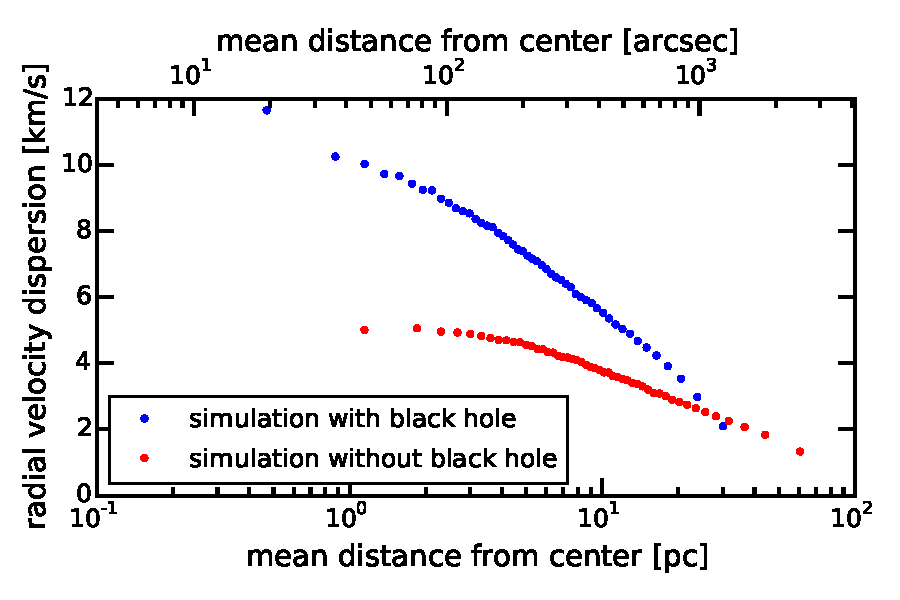
\includegraphics[width=\textwidth]{Plots/radial_velocity_dispersion.pdf}
		\caption{Radial velocity dispersions}
		\label{[fig:radial_vel_disp]}
	\end{subfigure}
	\hfill
	\begin{subfigure}{0.475\textwidth}
		\centering
		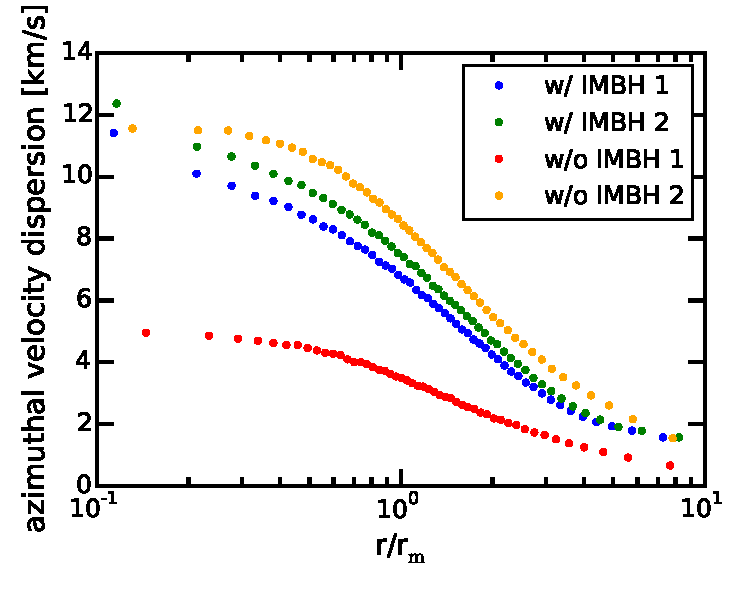
\includegraphics[width=\textwidth]{Plots/azimuthal_velocity_dispersion.pdf}
		\caption{Azimuthal velocity dispersions}
		\label{[fig:azimuthal_vel_disp]}
	\end{subfigure}
	\vskip\baselineskip
	\begin{subfigure}{0.475\textwidth}
		\centering
		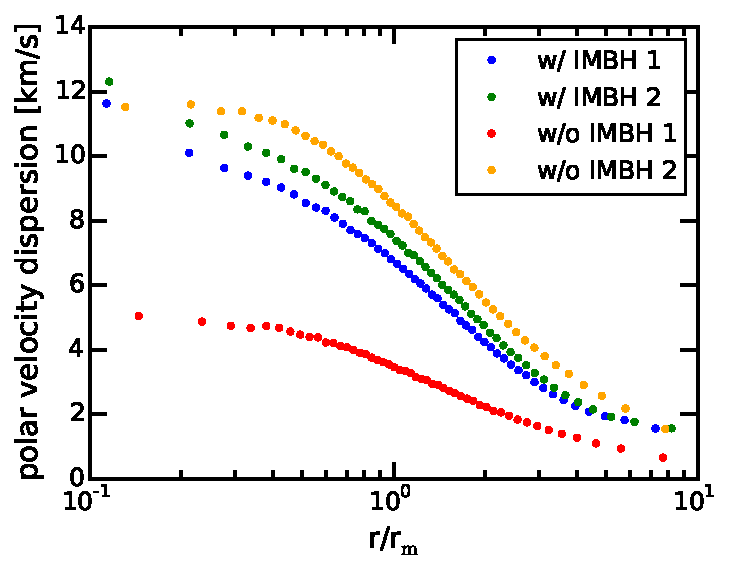
\includegraphics[width=\textwidth]{Plots/polar_velocity_dispersion.pdf}
		\caption{Polar velocity dispersions}
		\label{[fig:polar_vel_disp]}
	\end{subfigure}


	\caption{Velocity dispersion profiles as a function of the radius in units of the effective radius \(\mathrm{r_{eff}}\). They are binned in a way that each bin contains the same amount of stars. We can see that the velocity dispersion of the simulation with \ac{IMBH} rises towards the centre whereas the simulation without \ac{IMBH} exhibits a cored profile.}
\end{figure*}
As expected there is a rise in the centre for the simulation with \ac{IMBH}. This is due the high gravitational potential of the \ac{IMBH} which disturbs the dynamics of close stars. 


\subsubsection{Anisotropy}
Anisotropy can be calculated from (2) in \ref{sec2.1}. It is binned the same way as for the velocity dispersion and again dependent on the effective radii.
\begin{figure}
	\centering
	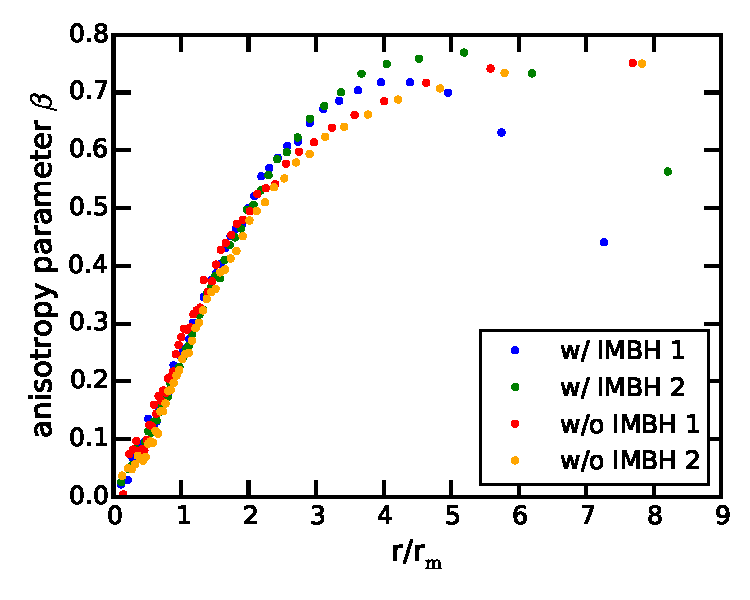
\includegraphics[width=0.475\textwidth]{Plots/anisotropy_parameter_beta.pdf}
	\caption{Anisotropy parameter \(\beta\). Both simulations are radial anisotropic. The simulation with \ac{IMBH} has a peak at 4 effective radii where it is most radial anisotropic. The other simulation is rising until the end. The far more outside a star is the higher its radial anisotropy is.}
	\label{fig:anisotropy_param}
\end{figure}
In the center of both \acp{GC} there is nearly the same anisotropy. Both are positive and rising. That means the systems are radial anisotropic. The \ac{GC} with \ac{IMBH} is most radial anisotropic in its center at about 4 effective radii. The other \ac{GC} is becoming more radial anisotropic the more far from the centre it is.

\subsubsection{Density profile}
The density profile shows the density of the system over its radius. The bins are chosen so that the radii are equidistant on a logarithmic scale and that they are at least 100 stars per bin to have a reliable stochastic. Outside of the cluster the density is set to 0. In the innermost part the density is set to be as the innermost point.
plots\\
\begin{figure}
	\centering
	\begin{subfigure}{0.475\textwidth}
		\centering
		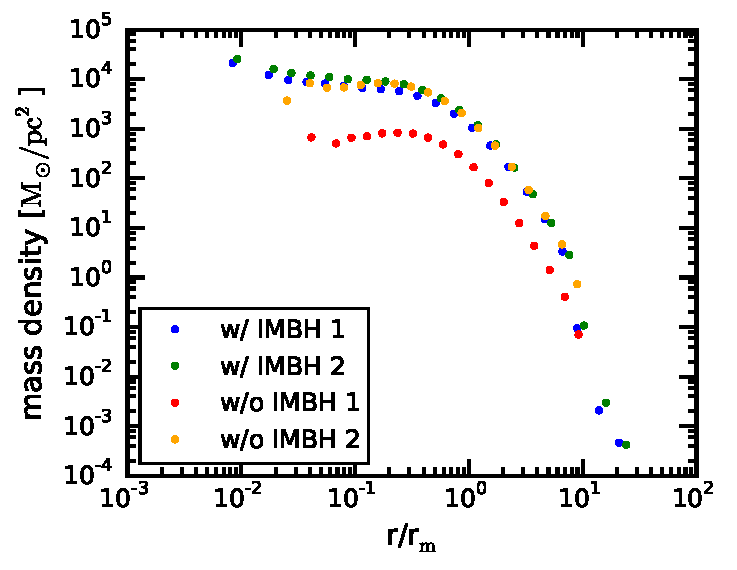
\includegraphics[width=\textwidth]{Plots/density_profiles.pdf}
		\caption{Mass density profiles of all four simulations.}
		\label{mass_dens_points}
	\end{subfigure}
	\hfill
	\begin{subfigure}{0.475\textwidth}
		\centering
		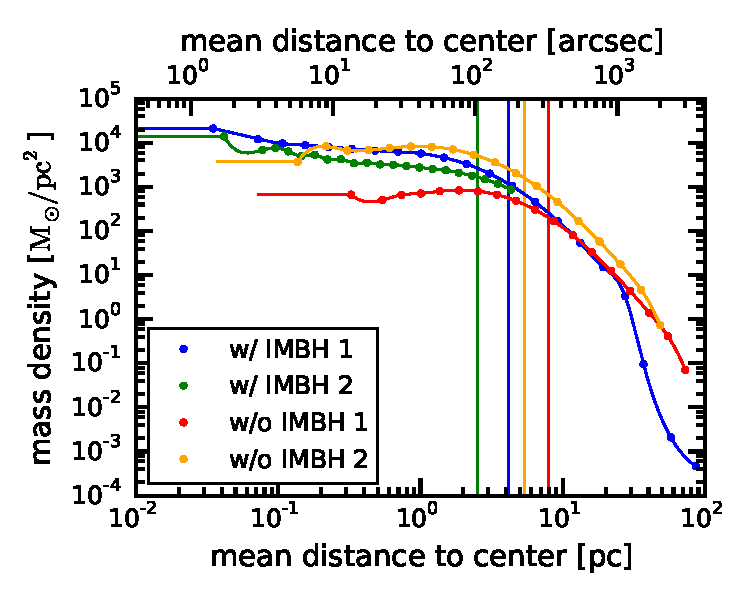
\includegraphics[width=\textwidth]{Plots/density_profiles_interpolated.pdf}
		\caption{Interpolated mass density profiles of SIM 1 and SIM 3.}
		\label{mass_dens_intpol}
	\end{subfigure}
	\caption{Mass density profiles. The density in \(\frac{M_{\odot}}{pc^2}\) is plotted against the effective radius. The density of the \ac{GC} with \ac{IMBH} is everywhere larger than the density of the \ac{GC} without \ac{IMBH}. In the centre there is a raise in the density of the \ac{GC} with \ac{IMBH} whereas the other \ac{GC} stays approximately on the same level. Both start decreasing at about 0.5 \(\mathrm{r_eff}\).}
	\label{fig:mass_density_profile}
\end{figure}

\subsubsection{Potential}
From the density profile we can compute the potential as described in \ref{dens_pot_theory}. It is composed by the potential given from the stars and if there is one the potential of the \ac{IMBH} expressed as Kepler potential.
\begin{figure}
	\centering
	\includegraphics[width=0.475\textwidth]{Plots/Pot.pdf}
	\caption{Potential of all \acp{GC}. SIM 1 and SIM 2 are nearly overlaying. They are the same simulation at different ages. The simulation lost 5 \% of it's stars with 10 \% of the total mass while the \ac{IMBH} gained 13 \%. The potential of the stars declines while the potential of the \ac{IMBH} rises so the potential stays the same. The \acp{GC} without \ac{IMBH} remain constant in the inner part (until 0.5 half mass radii) and decrease from the points where their densities decrease.}
\end{figure}


\subsection{Investigations of orbits in action space}
wilma class 
\subsubsection{Orbits \& actions}

\subsubsection{Integral of motions along orbits}
